\documentclass[10pt,aspectratio=169]{beamer}
\usetheme{Boadilla}
\usepackage{graphicx,booktabs,tikz,array}
\usetikzlibrary{arrows.meta,positioning,calc}
\definecolor{ModelNavy}{HTML}{244A73}
\definecolor{ModelTeal}{HTML}{008575}
\definecolor{ModelRed}{HTML}{BC5046}
\setbeamercolor{structure}{fg=ModelNavy}
\setbeamercolor{frametitle}{bg=ModelNavy,fg=white}
\setbeamercolor{title}{fg=ModelNavy}
\setbeamertemplate{navigation symbols}{}
\setbeamertemplate{footline}[frame number]
\setbeamersize{text margin left=0.65cm,text margin right=0.65cm}
\setbeamertemplate{itemize items}[circle]
% \graphicspath{{final-presentation-figures/}{reports/final-presentation-figures/}}
% \IfFileExists{final-presentation-figures/numbers.tex}{\input{final-presentation-figures/numbers.tex}}{\input{reports/final-presentation-figures/numbers.tex}}
\newcommand{\source}[1]{\par\vspace{1mm}{\tiny\color{gray}#1}}
\newcommand{\takeaway}[1]{\par\smallskip{\color{ModelTeal}\bfseries #1}\par\smallskip}
\providecommand{\MeanEstimate}{\ldots}
\providecommand{\MaxEstimate}{\ldots}
\providecommand{\MeanPredict}{\ldots}
\tikzset{box/.style={draw=ModelNavy,rounded corners,fill=ModelNavy!5,align=center,minimum height=0.8cm,font=\small},arr/.style={-{Stealth},thick,ModelNavy}}
\title{Quantum Circuit Runtime Inference}
\subtitle{SC Quantathon v3}
\date{}
\author{Team ``Hit the Quant''}
\begin{document}

\begin{frame}
\titlepage
\end{frame}

\begin{frame}{The Problem}
\begin{itemize}
\item \textbf{Schedule jobs:} Useful for separating out short runs from long runs
\item \textbf{Plan capacity:} Can be used to estimate queue time and CPU demand for customers
\item \textbf{Screen expensive jobs:} Flags jobs with excessive runtime before launch
\item \textbf{Compare settings:} Estimate runtime for each of the supported thresholds
\end{itemize}

Good estimation can lead to fewer failed jobs, better completion-time estimates, and less wasted compute.
\end{frame}

\begin{frame}{The Challenge}
\begin{itemize}
\item \textbf{Input:} OpenQASM circuit + simulator threshold.
\begin{itemize}
\item Threshold controls tradeoff between efficiency/accuracy
\end{itemize}
\item \textbf{Output:} estimated runtime of program
\item \textbf{Constraints:} 15-second limit for each circuit
\end{itemize}\par
\vspace{1em}
\centering
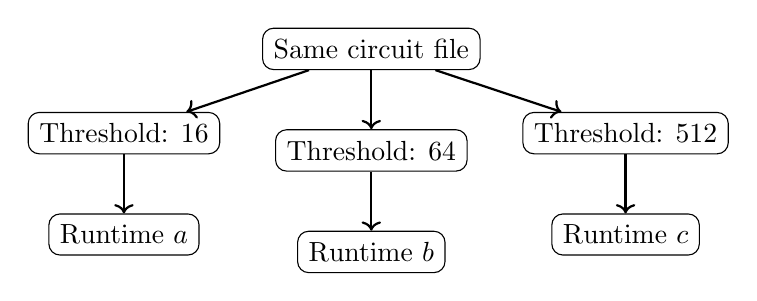
\begin{tikzpicture}[node distance=0.75cm,
    box/.style={draw, rectangle, rounded corners, align=center, inner sep=4pt},
    arr/.style={->, thick}]
    
% first level
\node[box] (a) {Same circuit file};

% second level – three thresholds
\node[box, below left=of a] (b1) {Threshold: 16};
\node[box, below=of a]      (b2) {Threshold: 64};
\node[box, below right=of a] (b3) {Threshold: 512};

% third level – three runtimes
\node[box, below=of b1] (c1) {Runtime $a$};
\node[box, below=of b2]      (c2) {Runtime $b$};
\node[box, below=of b3] (c3) {Runtime $c$};

% arrows
\draw[arr] (a) -- (b1);
\draw[arr] (a) -- (b2);
\draw[arr] (a) -- (b3);

\draw[arr] (b1) -- (c1);
\draw[arr] (b2) -- (c2);
\draw[arr] (b3) -- (c3);
\end{tikzpicture}\par
\smallskip
\end{frame}

\begin{frame}{Training Data}
\centering
\includegraphics[width=.87\textwidth,height=4.45cm,keepaspectratio]{assets/training_data_summary.png}
\begin{itemize}
\item \textbf{532 circuits files; 1,497 labels:} 1,464 completed runs and 33 timeouts.
\item Provided with circuit ID, threshold, duration/status
\item Fixed information: backend (CPU simulator), single precision, shots
\end{itemize}
\end{frame}

\begin{frame}
    \vspace*{\fill}        % push content to vertical centre
    \centering
    {\Huge Tested Workflows}\\[1.5ex]   % huge, bold, centered
    \vspace*{\fill}
\end{frame}

\begin{frame}{Tested Workflows: Gaussian Mixture Model}
\centering
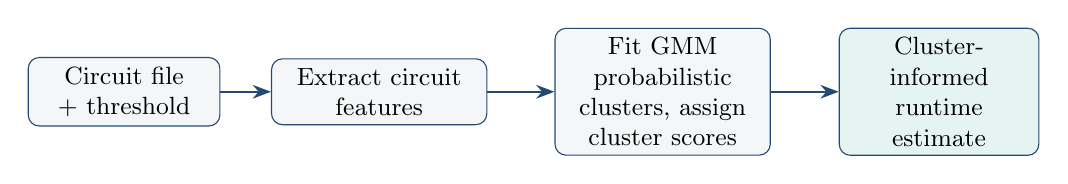
\begin{tikzpicture}[x=.9cm,y=1cm]
\node[box,text width=2.2cm] (input) at (0,0) {Circuit file\\+ threshold};
\node[box,text width=2.5cm] (features) at (3.6,0) {Extract circuit\\features};
\node[box,text width=2.5cm] (gmm) at (7.6,0) {Fit GMM probabilistic clusters, assign cluster scores};
\node[box,text width=2.3cm,fill=ModelTeal!10] (runtime) at (11.5,0) {Cluster-informed\\runtime estimate};
\draw[arr] (input)--(features); \draw[arr] (features)--(gmm); \draw[arr] (gmm)--(runtime);
\end{tikzpicture}
\vspace{.25cm}
\begin{itemize}
\item GMM groups circuits with similar measured runtime patterns; probabilities express uncertain cluster membership.
\item Use the identified groups to characterize runtime behavior across circuit settings.
\end{itemize}
\end{frame}

\begin{frame}{Tested Workflows: Graph Transformer}
\centering
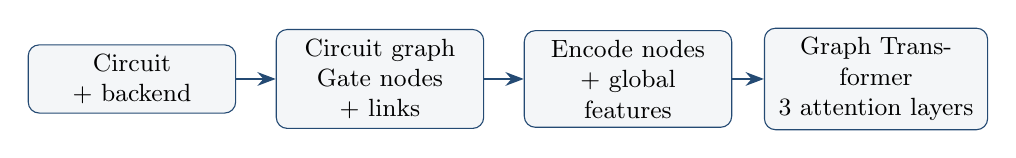
\begin{tikzpicture}[x=.9cm,y=1cm]
\node[box,text width=2.4cm] (input) at (0,0) {Circuit\\+ backend};
\node[box,text width=2.4cm] (repr) at (3.5,0) {Circuit graph\\Gate nodes + links};
\node[box,text width=2.4cm] (features) at (7.0,0) {Encode nodes\\+ global features};
\node[box,text width=2.6cm] (gt) at (10.5,0) {Graph Transformer\\3 attention layers};
\draw[arr] (input)--(repr); \draw[arr] (repr)--(features); \draw[arr] (features)--(gt);
\end{tikzpicture}
\vspace{.25cm}
\begin{itemize}
\item Workflow based on Ma \& Li, \emph{Understanding and Estimating the Execution Time of Quantum Circuits} (arXiv:2411.15631v2).
\item Graph features capture gate connectivity and global features summarize circuit size and gate counts.
\item Combines pooled graph features with global features in a neural regressor.
\end{itemize}
\end{frame}

\begin{frame}{Tested Workflows: $k$-Nearest Neighbors}
\centering
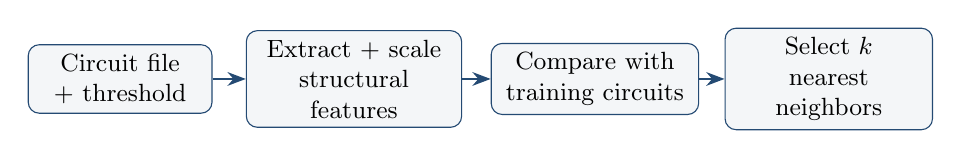
\begin{tikzpicture}[x=.9cm,y=1cm]
\node[box,text width=2.1cm] (input) at (0,0) {Circuit file\\+ threshold};
\node[box,text width=2.5cm] (features) at (3.3,0) {Extract + scale\\structural features};
\node[box,text width=2.4cm] (distance) at (6.7,0) {Compare with\\training circuits};
\node[box,text width=2.4cm] (neighbors) at (10.0,0) {Select $k$\\nearest neighbors};
\draw[arr] (input)--(features); \draw[arr] (features)--(distance); \draw[arr] (distance)--(neighbors);
\end{tikzpicture}
\vspace{.25cm}
\begin{itemize}
\item Neighbor similarity is computed from the circuit features and settings.
\item Nearby labeled circuits provide the runtime estimate.
\end{itemize}
\end{frame}

\begin{frame}{Tested Workflows: ExtraTrees + Regression Model}
\centering
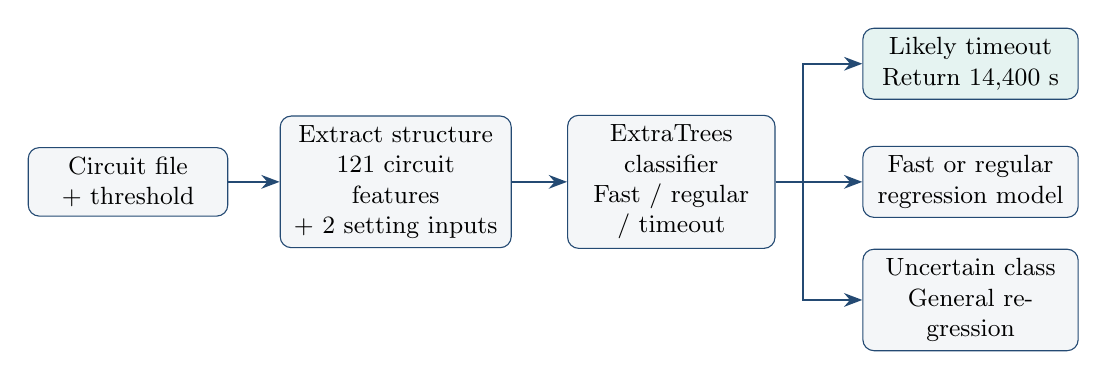
\begin{tikzpicture}[x=1cm,y=1cm]
\node[box,text width=2.3cm] (input) at (0,0) {Circuit file\\+ threshold};
\node[box,text width=2.7cm] (features) at (3.4,0) {Extract structure\\121 circuit features\\+ 2 setting inputs};
\node[box,text width=2.4cm] (class) at (6.9,0) {ExtraTrees classifier\\Fast / regular / timeout};
\node[box,text width=2.5cm,fill=ModelTeal!10] (timeout) at (10.7,1.5) {Likely timeout\\Return 14,400 s};
\node[box,text width=2.5cm] (expert) at (10.7,0) {Fast or regular\\regression model};
\node[box,text width=2.5cm] (fallback) at (10.7,-1.5) {Uncertain class\\General regression};
\draw[arr] (input)--(features); \draw[arr] (features)--(class);
\draw[arr] (class.east)--++(.35,0)|-(timeout.west);
\draw[arr] (class)--(expert);
\draw[arr] (class.east)--++(.35,0)|-(fallback.west);
\end{tikzpicture}
\vspace{.25cm}
\begin{itemize}
\item \textbf{ExtraTrees:} many randomized decision trees combine their estimates.
\item Classifier routes the job and a specialist estimates duration on a log scale
\end{itemize}
\end{frame}

\begin{frame}{Tested Workflows: Mock Simulator + Neural Network}
\centering
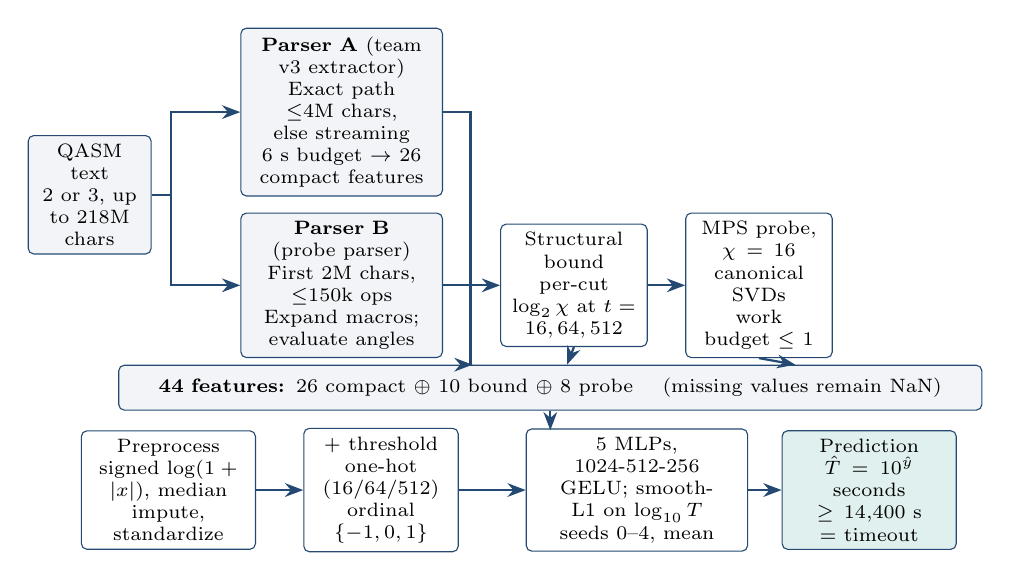
\begin{tikzpicture}[x=1cm,y=1cm,>=Stealth,
  flow/.style={draw=ModelNavy,rounded corners=2pt,fill=ModelNavy!6,align=center,
    font=\scriptsize,inner sep=3pt,minimum height=0.68cm},
  stage/.style={draw=ModelNavy,rounded corners=2pt,fill=white,align=center,
    font=\scriptsize,inner sep=3pt,minimum height=0.72cm},
  link/.style={-{Stealth},thick,ModelNavy},
  tag/.style={font=\scriptsize\bfseries,text=ModelNavy}]
% Feature extraction branches
\node[flow,text width=1.35cm] (qasm) at (.85,2.5) {QASM text\\2 or 3, up to 218M chars};
\node[flow,text width=2.35cm] (parsera) at (4.05,3.55) {\textbf{Parser A} (team v3 extractor)\\Exact path $\leq$4M chars, else streaming\\6 s budget $\to$ 26 compact features};
\node[flow,text width=2.35cm] (parserb) at (4.05,1.35) {\textbf{Parser B} (probe parser)\\First 2M chars, $\leq$150k ops\\Expand macros; evaluate angles};
\node[stage,text width=1.65cm] (bound) at (7.0,1.35) {Structural bound\\per-cut $\log_2\chi$ at $t=16,64,512$};
\node[stage,text width=1.65cm] (mps) at (9.35,1.35) {MPS probe, $\chi=16$\\canonical SVDs\\work budget $\leq 1$};
\node[flow,text width=10.75cm,minimum height=.57cm] (features) at (6.7,.05) {\textbf{44 features:} 26 compact $\oplus$ 10 bound $\oplus$ 8 probe \quad (missing values remain NaN)};
\draw[link] (qasm.east)--++(.25,0)|-(parsera.west);
\draw[link] (qasm.east)--++(.25,0)|-(parserb.west);
\draw[link] (parserb)--(bound); \draw[link] (bound)--(mps);
\draw[link] (parsera.east)--++(.35,0)|-([xshift=4.5cm]features.north west);
\draw[link] (bound.south)--([xshift=5.7cm]features.north west);
\draw[link] (mps.south)--([xshift=8.6cm]features.north west);
% Prediction pipeline
\node[stage,text width=2.0cm] (prep) at (1.85,-1.25) {Preprocess\\signed $\log(1+|x|)$, median impute, standardize};
\node[stage,text width=1.75cm] (threshold) at (4.55,-1.25) {$+$ threshold\\one-hot (16/64/512)\\ordinal $\{-1,0,1\}$};
\node[stage,text width=2.6cm] (mlp) at (7.8,-1.25) {5 MLPs, 1024-512-256\\GELU; smooth-L1 on $\log_{10}T$\\seeds 0--4, mean};
\node[flow,text width=2.0cm,fill=ModelTeal!12] (prediction) at (10.75,-1.25) {Prediction\\$\hat T=10^{\hat y}$ seconds\\$\geq14{,}400$ s = timeout};
\draw[link] (features.south)--(features.south |- prep.north);
\draw[link] (prep)--(threshold); \draw[link] (threshold)--(mlp); \draw[link] (mlp)--(prediction);
\end{tikzpicture}
\end{frame}

\begin{frame}
    \vspace*{\fill}        % push content to vertical centre
    \centering
    {\Huge Final Model Statistics}\\[1.5ex]   % huge, bold, centered
    \vspace*{\fill}
\end{frame}

\begin{frame}{Model Runtime}
\centering
% \includegraphics[width=.92\textwidth,height=4.4cm,keepaspectratio]{estimation-speed.pdf}
\includegraphics[width=.87\textwidth,height=4.45cm,keepaspectratio]{assets/simulation_model_circuit_processing_time.png}
\takeaway{Mean extraction + one prediction: \MeanEstimate\ s\quad |\quad Maximum: \MaxEstimate\ s}
\begin{itemize}
\item Prediction takes a median 13 ms per call; features are reused across settings.
\item Measured across 532 circuits and 1,596 predictions on this local machine.
\end{itemize}
\end{frame}

\begin{frame}{Model Validation Scores}
\centering
% \includegraphics[width=.93\textwidth,height=4.6cm,keepaspectratio]{prediction-quality.pdf}
\includegraphics[width=.87\textwidth,height=4.45cm,keepaspectratio]{assets/r2_residual_diagnostic.png}
\begin{itemize}
\item \textbf{Challenge score: 94.81\%.} Grouped five-fold cross-validation; rewards small proportional errors.
\item \textbf{$R^2$: 0.806 in seconds; 0.960 in log seconds.} Completed runs; higher means better fit.
\end{itemize}
\end{frame}

\begin{frame}{Timeout Limitations}
\begin{columns}[T]
\column{.59\textwidth}
\includegraphics[width=.87\textwidth,height=4.45cm,keepaspectratio]{assets/timeout_detection.png}
\column{.38\textwidth}
\begin{itemize}
\item \textbf{10 of 33} timeouts predicted at or above the 4-hour cap.
\item \textbf{25 of 33} timeout predictions landed within $2\times$ of the cap; mean timeout score was 88.0\%.
\item \textbf{1 of 1,464} successful runs was predicted at or above the cap.
\item Cap predictions are a review signal; the model predicts runtime continuously.
\end{itemize}
\end{columns}
\end{frame}

\begin{frame}{Other Limitations and Future Experimentation}
\small
\begin{tabular}{@{}p{4.4cm}p{8.9cm}@{}}
\toprule
\textbf{Current limitation} & \textbf{Next exploration}\\\midrule
Rare long runs and severe misses & Have more long-run examples, audit the largest underestimates\\[3mm]
False timeout alarms & Tune the cost of missed timeouts versus false alarms\\[3mm]
Only one simulator environment & Collect labels for new hardware, precision, and shot counts; retrain before use\\[3mm]
\end{tabular}
\smallskip
\begin{itemize}
\item Experiment with different combinations of models to improve runtime predictions
\item Classifying jobs based on model strengths and routing it to the respective models
\item Testing with a larger dataset
\end{itemize}
\end{frame}

\appendix
\begin{frame}{Reference: Model Settings and Score Interpretation}
\begin{columns}[T]
\column{.54\textwidth}
\textbf{Final model}
\begin{itemize}
\item Architecture: 5-seed MLP ensemble (48--1024--512--256--1).
\item Fast class: none; predicts runtime continuously.
\item Timeout indicator: prediction $\geq 14{,}400$ s.
\end{itemize}
\column{.43\textwidth}
\textbf{Challenge scoring}
\[
 s=\max\left(0,1-\frac{|\log_{10}(\hat t/t)|}{2}\right)
\]
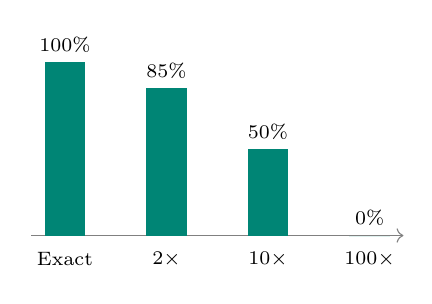
\begin{tikzpicture}[x=.43cm,y=.022cm]
\draw[->,gray] (0,0)--(11,0);
\foreach \x/\h/\lab/\val in {1/100/Exact/100,4/84.95/2$\times$/85,7/50/10$\times$/50,10/0/100$\times$/0}{
\fill[ModelTeal] (\x-.6,0) rectangle (\x+.6,\h);
\node[font=\scriptsize,above] at (\x,\h) {\val\%};
\node[font=\scriptsize,below] at (\x,-4) {\lab};}
\end{tikzpicture}
\end{columns}
\end{frame}
\end{document}
